\chapter{Project Details}

This chapter provides an in-depth explanation of the project's components and tools used. The system was developed using Swift, Xcode, RealityComposer Pro and the Object Capture app to leverage the capabilities of Apple Vision Pro.

% \section{UI/UX Design}
\section{UI/UX Design}
The application has a streamlined user interface with a single window navigating between different views to ensure an intuitive and user-friendly experience. Below is the flow of UI/UX interactions. Some parts of the interface were designed and implemented during the first semester. In the second semester, we expanded the system by integrating object tracking and annotation.

In addition to these modifications, button visuals were revised to provide a more professional appearance. (Figures \ref{fig:button_before} and \ref{fig:button_after} show the button appearance before and after the updates.)

\begin{figure}[h!]
    \centering
    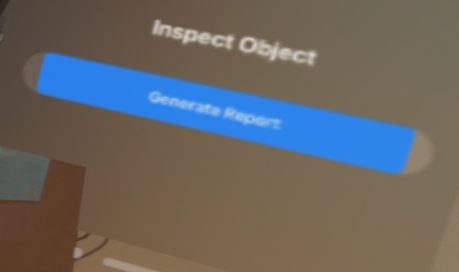
\includegraphics[width=0.4\textwidth]{button_before.png}
    \caption{\centering Button appearance before visual update.}
    \label{fig:button_before}
\end{figure}

\begin{figure}[h!]
    \centering
    
\includegraphics[width=0.4\textwidth]{button_after.png}
    \caption{\centering Button appearance after visual update.}
    \label{fig:button_after}
\end{figure}

\subsection{Initial Session Start}
The application starts with a view prompting the user to begin an ARKit session. In the first semester, this session was primarily responsible for initializing plane detection and world tracking. In the current version, it also starts object tracking for all referenced objects. The interface provides visual indicators to guide the user during this setup phase. (Figure \ref{fig:ui_session_start} shows the UI at this stage.)
\begin{figure}[H]
    \centering
    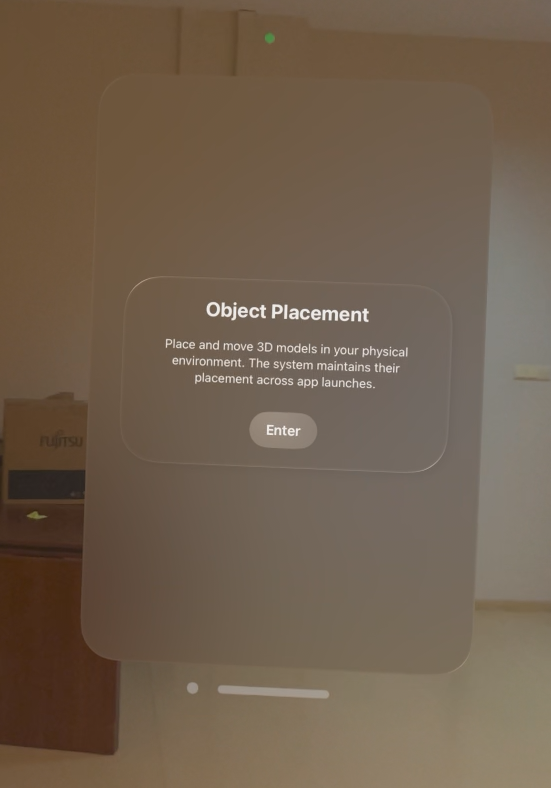
\includegraphics[width=0.37\textwidth]{session_start_ui.png} % Replace with your image file name
    \caption{UI for starting the ARKit session.}
    \label{fig:ui_session_start}
\end{figure}

\subsection{Object Selection Menu}
After initializing the session, the user is directed to an object selection menu. In this view:
\begin{itemize}
    \item The user selects an object from the available options.
    \item When an object is clicked, the \texttt{selectedObject} state is updated.
    \item The selected object is prepared for placement. (Figure \ref{fig:ui_object_selection} shows the object selection menu.)
\end{itemize}

While the basic selection mechanism was implemented in the first semester, this semester we expanded the menu by adding new models specifically designed to demonstrate the object tracking feature. Each of these new models is associated with a reference object file used for object recognition, along with a corresponding USDZ format 3D model for rendering in AR.

\begin{figure}[h!]
    \centering
    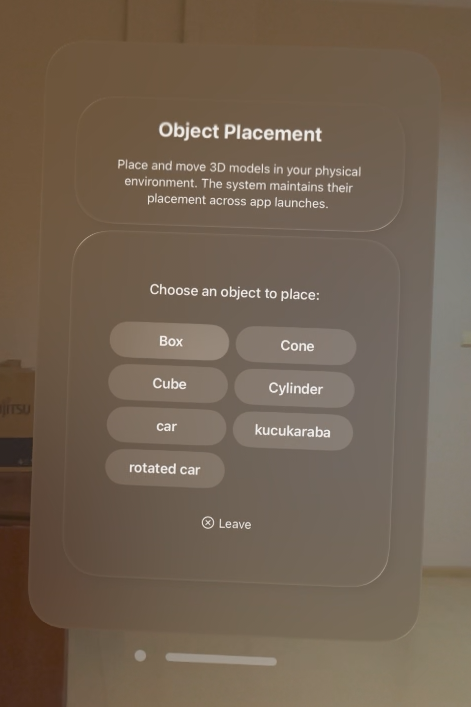
\includegraphics[width=0.4\textwidth]{object_selection_ui.png} % Replace with your image file
    \caption{Object selection menu UI.}
    \label{fig:ui_object_selection}
\end{figure}

\subsection{Initial Object Placement}
This component was implemented during the first semester and remains unchanged in the current version. During the initial placement of the selected object:
\begin{itemize}
    \item Placement tooltips are displayed to guide the user on positioning the object accurately.
    \item Visual aids ensure the user understands how to interact with the AR environment. (Figure \ref{fig:ui_initial_placement} shows the placement tooltip.)
\end{itemize}
\begin{figure}[H]
    \centering
    
\includegraphics[width=0.4\textwidth]{object_placement_tooltips.png} % Replace with your image file
    \caption{Placement tooltips during initial object placement.}
    \label{fig:ui_initial_placement}
\end{figure}

\subsection{Object Interaction View}
If there is already a placed object, the application navigates directly to the object interaction view. This view was initially developed in the first semester to support repositioning, inspection, and removal of the placed object. In the second semester, this view was extended with additional functionality, including a new annotation interaction feature and the relocation of the \textit{Generate Report} button.

\begin{itemize}
    \item The user can perform repositioning, inspection, annotation, report generation, or removal of the placed object. The interface displays buttons for these actions, as shown in Figure \ref{fig:object_interaction_view}.
\end{itemize}

\begin{figure}[H]
    \centering
    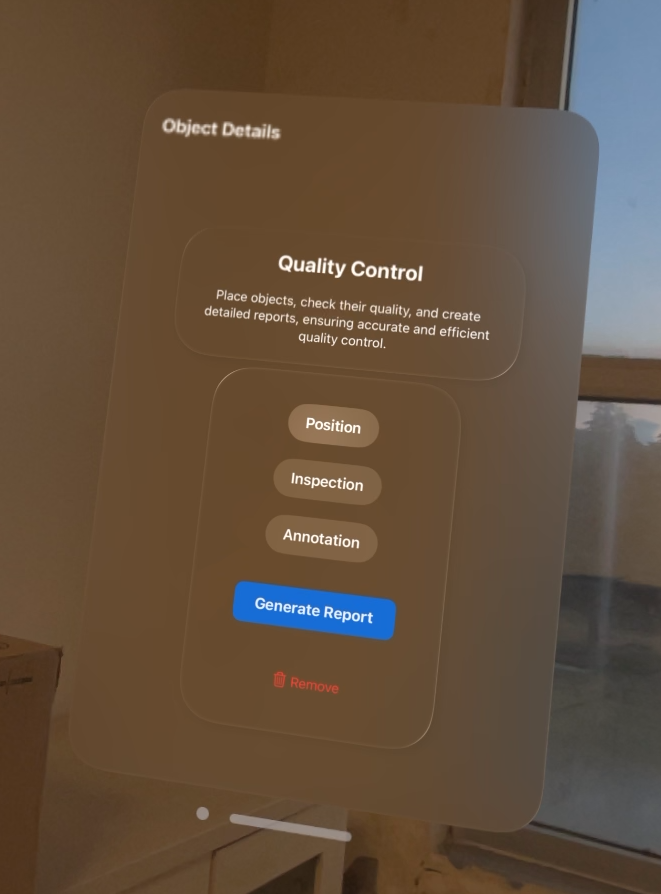
\includegraphics[width=0.39\textwidth]{object_interaction_view.png}
    \caption{\centering UI showing the buttons for repositioning, inspection, annotation, report generation, and removal.}
    \label{fig:object_interaction_view}
\end{figure}


\begin{itemize}
    \item Action buttons allow the user to activate the following functionalities:
    \begin{itemize}

        \item \textbf{Repositioning:} Includes rotation, left/right movement, and forward/backward movement. The user can use pinch and drag gestures (thumb and index finger) to perform the action. Only one action can be performed at a time.

        In addition to these basic controls, we introduced new buttons in the second semester to support object tracking visualization:
        \begin{itemize}
            \item \textbf{Snap Button:} Allows the user to align the placed model with the most recent object tracking data.
            \item \textbf{Object Tracking Mode Toggle:} Enables a continuous tracking mode where the model automatically updates its position and orientation according to real-time object tracking data.
        \end{itemize}

        These buttons are only visible when the selected model includes a valid reference object file and when the corresponding real-world object is detected in the environment.

        (Figure \ref{fig:ui_repositioning} shows the repositioning process and interaction layout.)
        \begin{figure}[H]
            \centering
            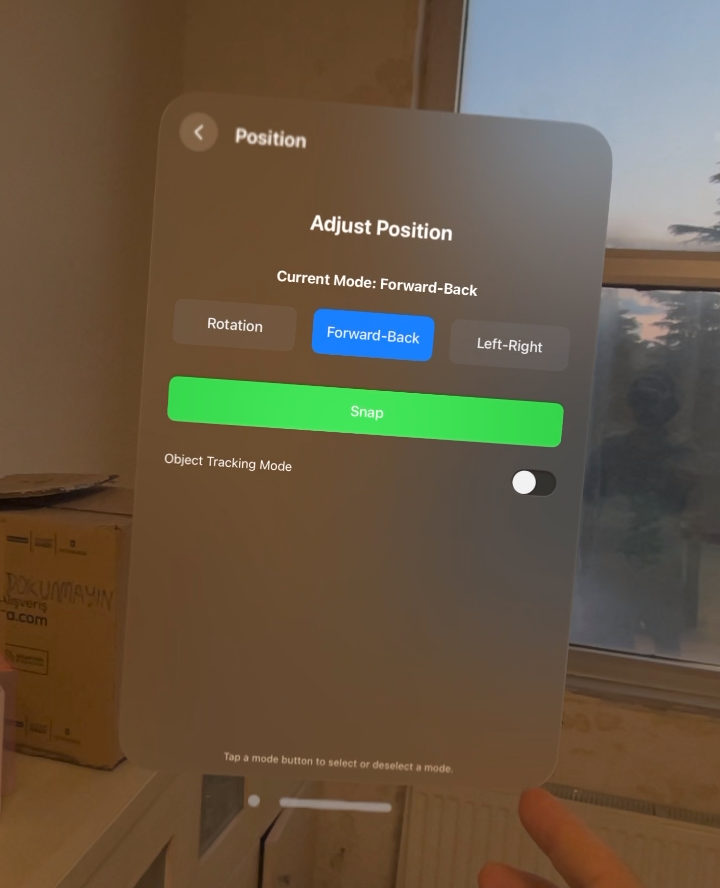
\includegraphics[width=0.47\textwidth]{repositioning_ui_new.png}
            \caption{\centering Repositioning view showing gesture-based controls and the newly added Snap and Tracking Mode buttons}
            \label{fig:ui_repositioning}
        \end{figure}


        \item \textbf{Inspection:} Inspection points are UI buttons attached to the placed object. These points activate only in the inspection view. Previously, this view included the \textit{Generate Report} button; however, in the current version, the button has been relocated to the main interaction view. (Figure \ref{fig:ui_inspection_view} shows the inspection view.)
        \begin{figure}[H]
            \centering
            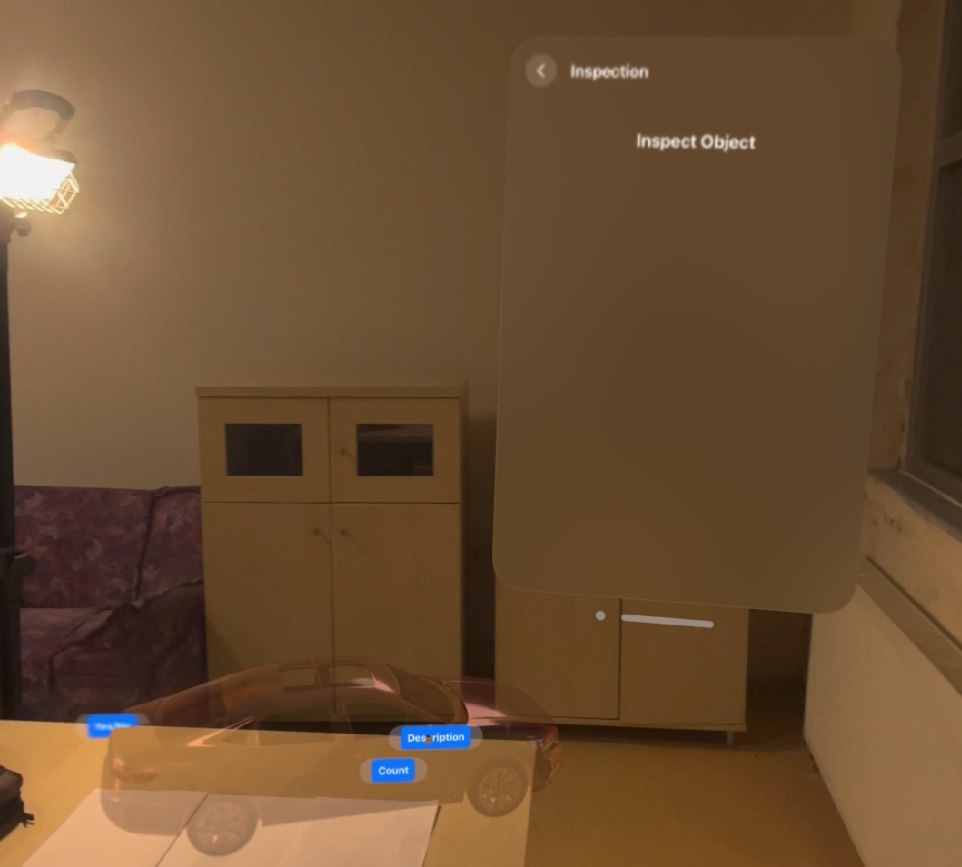
\includegraphics[width=0.6\textwidth]{inspection_view_ui.png}
            \caption{Inspection view showing active inspection points.}
            \label{fig:ui_inspection_view}
        \end{figure}

        \item \textbf{Annotation:} Introduced in the second semester, this feature allows the user to attach custom annotations directly onto the surface of the placed object. The user can tap on any point to create an annotation and enter relevant text. A search functionality is also included, enabling users to filter and locate annotations efficiently.

        \begin{figure}[H]
            \centering
            \begin{minipage}[t]{0.48\textwidth}
                \centering
                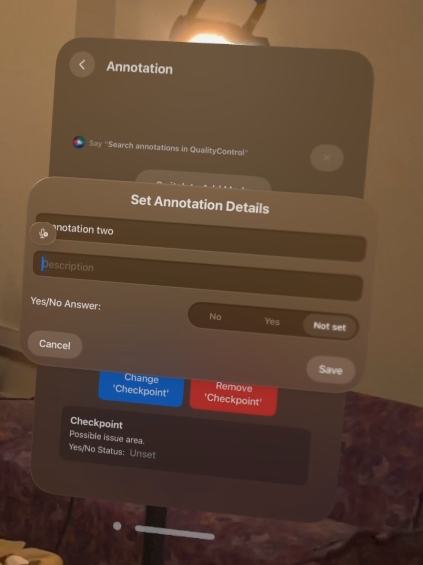
\includegraphics[width=\linewidth]{create_annotation.png}
                \caption{User creating an annotation on the object surface.}
                \label{fig:create_annotation}
            \end{minipage}
            \hfill
            \begin{minipage}[t]{0.48\textwidth}
                \centering
                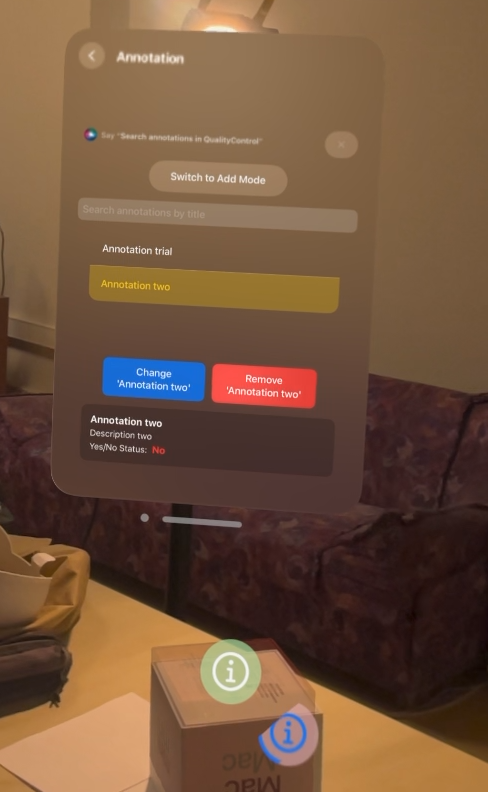
\includegraphics[width=\linewidth]{annotation_view.png}
                \caption{Annotation view showing the list of annotations attached to the object.}
                \label{fig:annotation_view}
            \end{minipage}
        \end{figure}



        \item \textbf{Generate Report:} Now placed directly within the object interaction view, this button triggers report generation without navigating away from the current screen. Upon activation, a confirmation message appears, indicating the report has been successfully generated. (Figure \ref{fig:generate_report_view} shows the confirmation message that appears after report generation.)
        \begin{figure}[H]
            \centering
            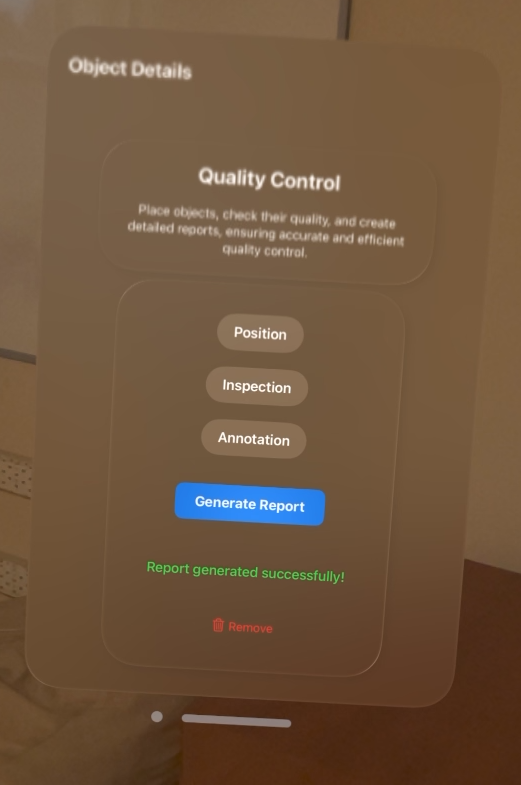
\includegraphics[width=0.4\textwidth]{generate_report_view.png}
            \caption{\centering Confirmation message indicating successful report generation.}
            \label{fig:generate_report_view}
        \end{figure}


        \item \textbf{Removal:} To remove the placed object, the user presses the remove button. A confirmation popup appears to ensure the action is intentional. (Figure \ref{fig:ui_remove_popup} shows the removal confirmation popup.)
        \begin{figure}[H]
            \centering
            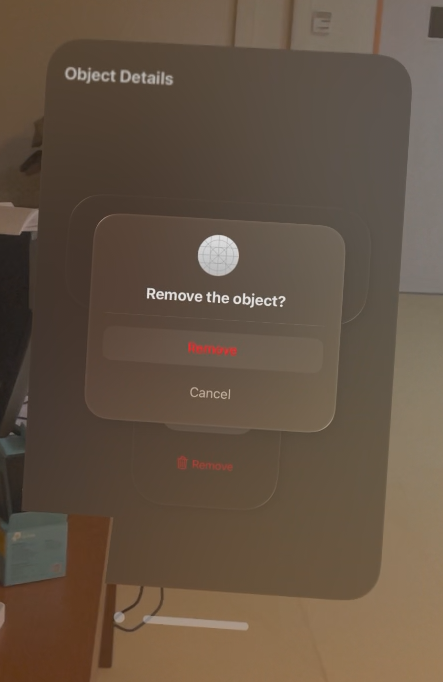
\includegraphics[width=0.4\textwidth]{remove_popup_ui.png}
            \caption{Confirmation popup for removing the placed object.}
            \label{fig:ui_remove_popup}
        \end{figure}
    \end{itemize}
\end{itemize}

\subsection{Inspection Detail View}
This component was fully implemented during the first semester and remains unchanged in the current version of the application. When an inspection point is clicked, the application navigates to the inspection detail view:
\begin{itemize}
    \item A question specific to the inspection point is displayed, which can be one of the following:
    \begin{itemize}
        \item Yes/No question.
        \item Count input.
        \item Description input.
    \end{itemize}
    \item The user provides the required input or feedback. (Figure \ref{fig:ui_inspection_detail} shows the inspection detail view.)
\end{itemize}


\begin{figure}[H]
    \centering
    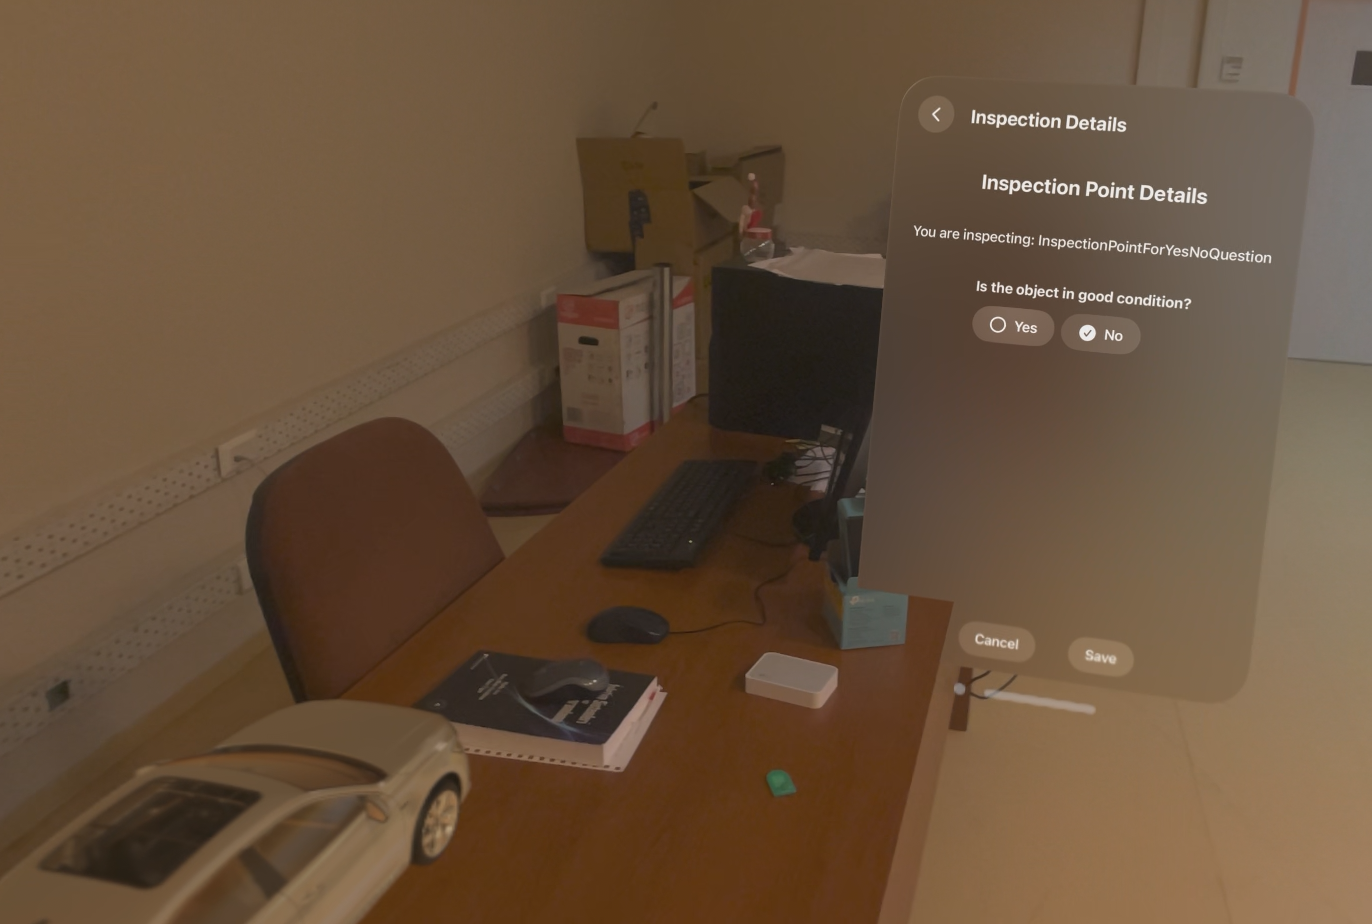
\includegraphics[width=0.8\textwidth]{inspection_detail_ui.png} % Replace with your actual file name
    \caption{Inspection detail view showing specific question types and input fields.}
    \label{fig:ui_inspection_detail}
\end{figure}

\subsection{Annotation Views}

In the second semester, an annotation system was introduced. This system uses visually responsive annotation cards that are spatially anchored to the 3D model and provide intuitive user interaction mechanisms.

\subsubsection{Annotation Card Design and Behavior}

Each annotation is represented by a UI card that is attached to a specific point on the 3D model. These cards remain anchored in space and are always oriented toward the user for readability. When the user gazes at a card, it activates a hover effect that expands the card to display more detailed information.

The expanded annotation card includes:
\begin{itemize}
    \item A \textbf{title} and \textbf{description} section.
    \item A \textbf{Yes/No} selection interface.
    
    The Yes/No state is visually encoded:
    \begin{itemize}
        \item \textbf{Green} for "Yes"
        \item \textbf{Red} for "No"
    \end{itemize}
\end{itemize}

\begin{figure}[H]
            \centering
            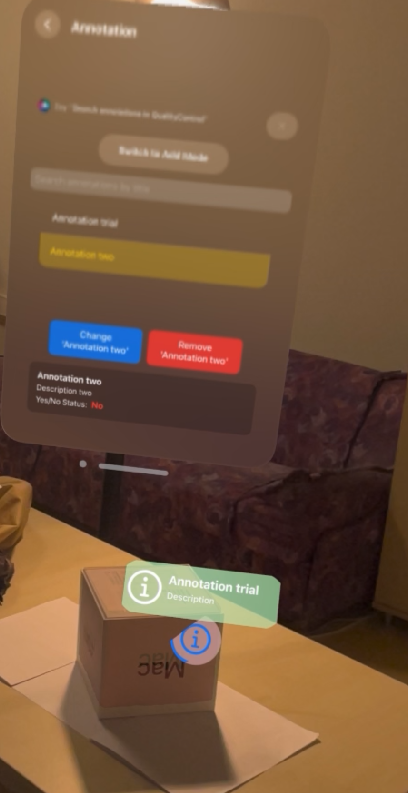
\includegraphics[width=0.4\textwidth]{annotation_card_design.png}
            \caption{Hovering annotation card design showing title, description, and Yes/No state.}
            \label{fig:annotation_card_design}
        \end{figure}

\subsubsection{Focused Annotation Mode}

There are multiple ways to activate this mode:
\begin{itemize}
    \item \textbf{Direct Focus:} The user can look at an annotation card in the AR scene and perform a pinch gesture to enter focused mode.
    \item \textbf{Menu-Based Activation:} Users can slide through a list of annotations displayed in the side menu. By looking at a list item and performing a pinch gesture, the corresponding annotation is automatically focused in the 3D view.
    \item \textbf{Search-Based Activation:} Users can search for an annotation using a built-in search bar. After locating the desired item, the user can look at it in the list and pinch to activate the focused annotation in the AR scene.
    \item \textbf{Siri Voice Search:} Users can also initiate a search by speaking to Siri. Siri automatically fills the search bar and highlights matching results in the list for pinch-based selection.
\end{itemize}

\begin{figure}[H]
            \centering
            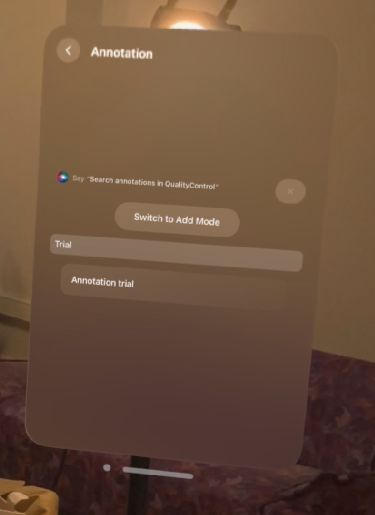
\includegraphics[width=0.4\textwidth]{annotation_search.png}
            \caption{\centering Search bar and list of annotations in the side menu. Users can search for annotations and select them to focus in the AR scene.}
            \label{fig:annotation_search}
        \end{figure}

When an annotation is focused, its card and the side menu visually changes to indicate the active state:
\begin{itemize}
    \item The annotation card turns \textbf{blue}, visually distinguishing it from other annotations in the scene.
    \item The user can then \textbf{edit} the annotation (e.g., update its title, description, or Yes/No state).
    \item The user also has the option to \textbf{remove} the focused annotation from the scene if it is no longer needed.
\end{itemize}

\begin{figure}[H]
            \centering
            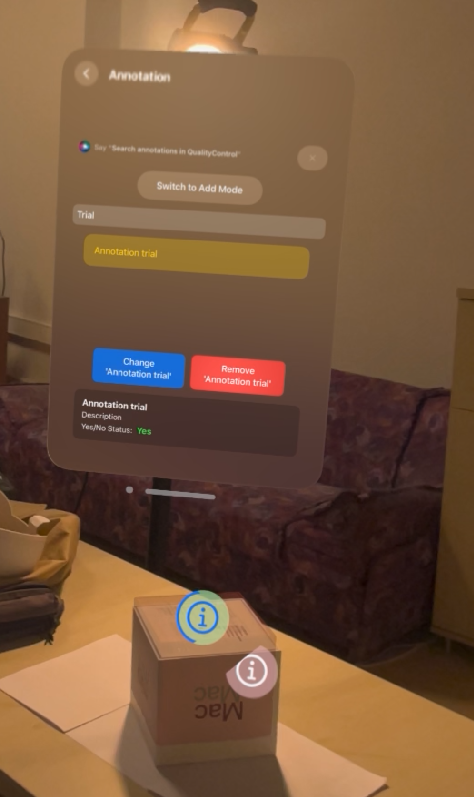
\includegraphics[width=0.4\textwidth]{annotation_focus.png}
            \caption{\centering Focused annotation card in the AR scene, showing the active state with a blue color. The user can edit or remove the annotation.}
            \label{fig:annotation_focus}
        \end{figure}




\section{Model Alignment and Object Tracking}

The system leverages ARKit’s capabilities for world tracking and plane detection to enable accurate model alignment and placement. Horizontal planes are specifically chosen to detect ground planes, ensuring precise object placement in the AR environment.

The 3D models used in the application are in the USDZ format, which is optimized for AR experiences on Apple devices.

In the second semester, we enhanced the model alignment system by integrating \textbf{object tracking} to allow more accurate and efficient placement of virtual objects in the AR environment. This feature complements ARKit’s existing plane detection and world tracking by aligning models directly to recognized real-world objects.

Additionally, to visually verify the precision of object alignment, \textbf{all 3D models were made semi-transparent and tinted red}. This visual modification enables users to inspect how accurately the virtual model overlays the physical object beneath it.


\subsection{Initial Placement}
This feature was implemented in the first semester and remains unchanged in the current version. During initial placement, the user is provided with a preview of the selected object. The preview is displayed as a greyed-out version of the object accompanied by a placement tooltip to guide the user in positioning it accurately. This feature allows the user to visually align the object with the detected ground plane before finalizing its placement, as shown in Figure \ref{fig:ui_initial_placement}.

To ensure that objects fit appropriately within the environment, size adjustments are made to the USDZ 3D models using SceneKit.

\subsection{Replacement}
This feature was introduced in the first semester and has been expanded in the second semester with additional object tracking functionality. If the user needs to reposition an already placed object, they can do so in the position mode of the application. In this mode:
\begin{itemize}
    \item The user can perform object rotation, as well as left/right and forward/backward movements.
    \item These adjustments are enabled only when the position mode is activated in the position view.
    \item Pinch and drag gestures (thumb and index finger) are used to perform these actions, as shown in Figure \ref{fig:ui_repositioning}.
    \item Two new buttons were added:
    \begin{itemize}
        \item \textbf{Snap Button:} Aligns the virtual model with the most recent object tracking data from ARKit.
        \item \textbf{Object Tracking Mode Toggle:} Continuously updates the model’s position and orientation using live tracking data when enabled.
    \end{itemize}
\end{itemize}

\subsection{Object Tracking}
To enable object tracking, each tracked model is paired with a reference object file in addition to its USDZ representation. These reference object files were generated using Xcode’s machine learning tool, which extracts object recognition data from the USDZ models.

We used iPhone Pro models equipped with LiDAR sensors to improve the accuracy of 3D reconstruction. This provided better depth data and enabled the creation of more reliable reference objects.

Textured and visually distinct objects were intentionally chosen to support more robust detection and tracking performance.

% Explanation about inspection will go here.
\section{Inspection}

All inspection operations, including providing input to inspection points and viewing inspection points, occur exclusively within the \textbf{Inspection View}. If the application is not in the \textbf{Inspection View}, all inspection points are removed from the interface. When the user navigates back to the \textbf{Inspection View}, the inspection points are dynamically regenerated (as shown in Figure \ref{fig:ui_inspection_view}).

To prevent user confusion or potential issues (e.g., uncertainty about whether data is saved), all inspection points are also removed when the application navigates to the \textbf{Inspection Detail View}. This design decision ensures reliability and eliminates bugs arising from unclear save states or interactions (as shown in Figure \ref{fig:ui_inspection_detail}).

The inspection system was fully implemented in the first semester and remains unchanged in the current version, with the exception of the removal of the \textbf{Generate Report} button from the \textbf{Inspection View}. Report generation has been moved to the object interaction view.

\subsection{Inspection Points}
For each inspection point on the placed model, a UI button is displayed (as shown in Figure \ref{fig:ui_inspection_view}). These buttons are dynamically positioned based on the specific locations of the inspection points on the model. When the user clicks an inspection point button, the application navigates to the \textbf{Inspection Detail View}, where the selected inspection point can be reviewed and updated.

\subsection{Inspection Detail View}
In the \textbf{Inspection Detail View}, users can perform inspections on the selected point. The system supports three types of inspections:
\begin{itemize}
    \item \textbf{Yes/No:} A binary choice indicating whether the inspection criteria have been met, as shown in Figure \ref{fig:ui_inspection_detail}.
    \item \textbf{Count:} Allows the user to input the quantity of specific elements related to the inspection point.
    \item \textbf{Description:} Provides a text field for the user to enter detailed notes or comments about the inspection point.
\end{itemize}

% Explanation about the Annotation system will go here.

% Explanation about generating reports will go here.
\section{Report Generation}

The report generation functionality in this system is powered by the third-party C library \textbf{libxlsxwriter}, which facilitates the creation of Excel files. This feature enables users to export inspection reports, which are saved directly to the Apple Vision Pro's local directory for easy access. While the initial implementation in the first semester focused on exporting object and inspection point data, this semester the functionality was extended to include annotations in the report.

\subsection{Implementation Overview}
Each report file is named dynamically based on the object being inspected and a unique identifier to avoid conflicts.

\subsection{Report Content}
The generated report contains the following key information:
\begin{itemize}
    \item \textbf{Object Details:} The name, width, height, and depth of the inspected object are recorded in the report.
    \item \textbf{Inspection Points:} Each inspection point associated with the object is detailed in the report. For every inspection point, the following attributes are included:
    \begin{itemize}
        \item \textbf{Name:} The identifier of the inspection point.
        \item \textbf{Depending on The Type of Inspection:}
        \begin{itemize}
            \item \textbf{Count:} The quantity associated with the inspection point, if applicable.
            \item \textbf{Description:} Detailed notes or observations provided by the user.
            \item \textbf{Is Correct:} A binary value (Yes/No) indicating whether the inspection point meets the desired criteria.
        \end{itemize}
    \end{itemize}
    \item \textbf{Annotations} \textit{(Second Semester):} Annotation cards added to the object in the AR scene are also included in the report. For each annotation:
    \begin{itemize}
        \item \textbf{Title:} The title of the annotation.
        \item \textbf{Description:} Textual content describing the annotation.
        \item \textbf{Yes/No State:} Whether the annotation is marked "Yes" or "No."
    \end{itemize}
\end{itemize}

An example of the generated Excel report, including both inspection and annotation data, is shown in Figure \ref{fig:example_excel}.

\begin{figure}[H]
    \centering
    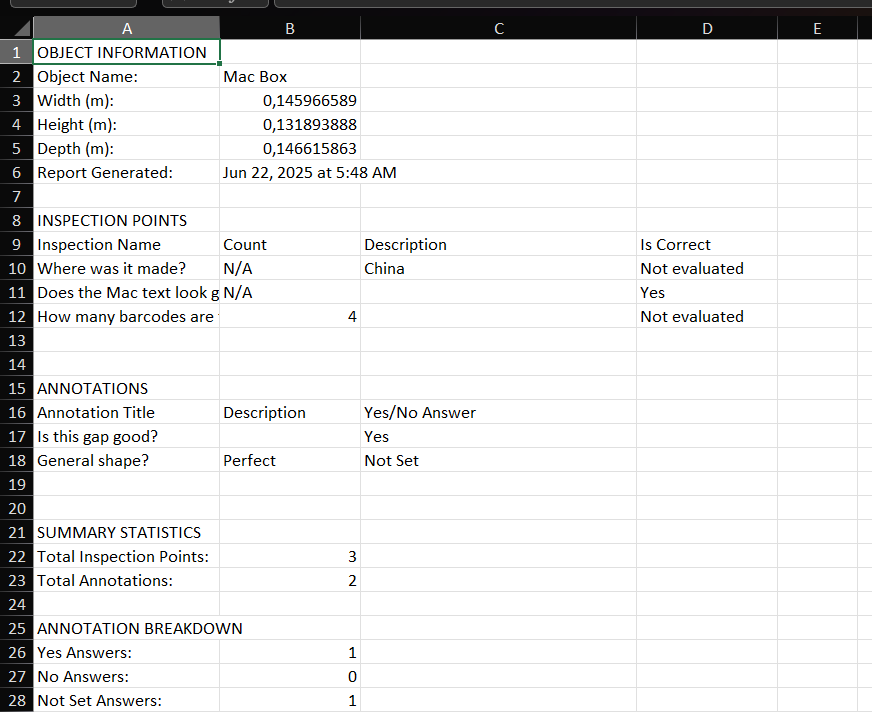
\includegraphics[width=0.8\textwidth]{example_excel.png} % Replace with your actual file name
    \caption{Example Excel report generated by the application, including inspection and annotation data.}
    \label{fig:example_excel}
\end{figure}
% \end{itemize}

% An example of the generated Excel report is shown in Figure \ref{fig:example_excel}.
% \begin{figure}[h!]
%     \centering
%     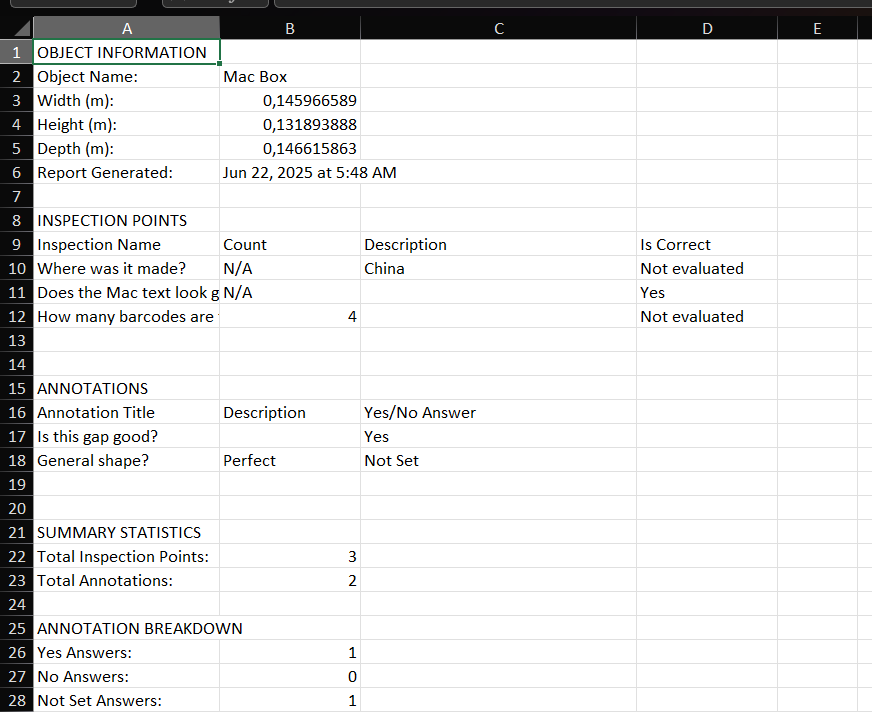
\includegraphics[width=0.8\textwidth]{example_excel.png} % Replace with your actual file name
%     \caption{Example Excel report generated by the application.}
%     \label{fig:example_excel}
% \end{figure}

\subsection{Integration with Apple Vision Pro}
The reports are stored locally on the Apple Vision Pro device, allowing users to access them conveniently through the file system. This integration ensures compatibility with the Vision Pro environment and leverages the device's capabilities for efficient data handling.

By using \textbf{libxlsxwriter}, the system provides a robust and efficient way to generate and manage detailed Excel reports, enhancing the overall functionality and usability of the quality control application.



\section{Use Case Diagram}
The use case diagram below illustrates the interaction between the user and the primary functionalities of the system.

\begin{landscape}
\begin{center}
    \begin{tikzpicture}[node distance=3cm, scale=0.8, transform shape]

        % Actor
        \node (user) [actor] {User};

        % Use cases
        \node (start) [usecase, below of=user, xshift=-10cm] {Start ARKit Session};
        \node (select) [usecase, below of=user, yshift=-10cm, xshift=-6cm] {Select Object};
        \node (place) [usecase, below of=user, yshift=-10cm, xshift=-2cm] {Place Object};
        \node (reposition) [usecase, below of=user, yshift=-10cm, xshift=2cm] {Reposition Object};
        \node (inspect) [usecase, below of=user, yshift=-10cm, xshift=6cm] {Inspect Object};
        \node (addanno) [usecase, below of=user, xshift=10cm] {Add Annotation};
        \node (report) [usecase, below of=user, xshift=14cm] {Generate Report};

         % Sub-use cases for ARKit session
        \node (tracking) [usecase, below of=start, xshift=-6cm, yshift=-2cm] {Object Tracking};
        \node (plane) [usecase, below of=start, xshift=-2cm, yshift=-2cm] {Plane Detection};
        \node (world) [usecase, below of=start, xshift=2cm, yshift=-2cm] {World Tracking};

        % Sub-use cases for Annotation
        \node (search) [usecase, below of=addanno, xshift=-2cm, yshift=-2cm] {Search Annotation (incl. Siri)};
        \node (focus) [usecase, below of=addanno, xshift=2cm, yshift=-2cm] {Focus Annotation};

        % Connections between actor and use cases
        \draw [->] (user) -- (start);
        \draw [->] (user) -- (select);
        \draw [->] (user) -- (place);
        \draw [->] (user) -- (reposition);
        \draw [->] (user) -- (inspect);
        \draw [->] (user) -- (addanno);
        \draw [->] (user) -- (report);
        
        % Relationships between use cases
        \draw [->] (start) -- node[midway, right] {includes} (tracking);
        \draw [->] (start) -- node[midway, right] {includes} (plane);
        \draw [->] (start) -- node[midway, right] {includes} (world);

         \draw [->] (addanno) -- node[midway, right] {includes} (search);
    \draw [->] (addanno) -- node[midway, right] {includes} (focus);

    \end{tikzpicture}
\end{center}
\end{landscape}

